\documentclass[twoside]{book}

% Packages required by doxygen
\usepackage{fixltx2e}
\usepackage{calc}
\usepackage{doxygen}
\usepackage[export]{adjustbox} % also loads graphicx
\usepackage{graphicx}
\usepackage[utf8]{inputenc}
\usepackage{makeidx}
\usepackage{multicol}
\usepackage{multirow}
\PassOptionsToPackage{warn}{textcomp}
\usepackage{textcomp}
\usepackage[nointegrals]{wasysym}
\usepackage[table]{xcolor}

% Font selection
\usepackage[T1]{fontenc}
\usepackage[scaled=.90]{helvet}
\usepackage{courier}
\usepackage{amssymb}
\usepackage{sectsty}
\renewcommand{\familydefault}{\sfdefault}
\allsectionsfont{%
  \fontseries{bc}\selectfont%
  \color{darkgray}%
}
\renewcommand{\DoxyLabelFont}{%
  \fontseries{bc}\selectfont%
  \color{darkgray}%
}
\newcommand{\+}{\discretionary{\mbox{\scriptsize$\hookleftarrow$}}{}{}}

% Page & text layout
\usepackage{geometry}
\geometry{%
  a4paper,%
  top=2.5cm,%
  bottom=2.5cm,%
  left=2.5cm,%
  right=2.5cm%
}
\tolerance=750
\hfuzz=15pt
\hbadness=750
\setlength{\emergencystretch}{15pt}
\setlength{\parindent}{0cm}
\setlength{\parskip}{3ex plus 2ex minus 2ex}
\makeatletter
\renewcommand{\paragraph}{%
  \@startsection{paragraph}{4}{0ex}{-1.0ex}{1.0ex}{%
    \normalfont\normalsize\bfseries\SS@parafont%
  }%
}
\renewcommand{\subparagraph}{%
  \@startsection{subparagraph}{5}{0ex}{-1.0ex}{1.0ex}{%
    \normalfont\normalsize\bfseries\SS@subparafont%
  }%
}
\makeatother

% Headers & footers
\usepackage{fancyhdr}
\pagestyle{fancyplain}
\fancyhead[LE]{\fancyplain{}{\bfseries\thepage}}
\fancyhead[CE]{\fancyplain{}{}}
\fancyhead[RE]{\fancyplain{}{\bfseries\leftmark}}
\fancyhead[LO]{\fancyplain{}{\bfseries\rightmark}}
\fancyhead[CO]{\fancyplain{}{}}
\fancyhead[RO]{\fancyplain{}{\bfseries\thepage}}
\fancyfoot[LE]{\fancyplain{}{}}
\fancyfoot[CE]{\fancyplain{}{}}
\fancyfoot[RE]{\fancyplain{}{\bfseries\scriptsize Generated by Doxygen }}
\fancyfoot[LO]{\fancyplain{}{\bfseries\scriptsize Generated by Doxygen }}
\fancyfoot[CO]{\fancyplain{}{}}
\fancyfoot[RO]{\fancyplain{}{}}
\renewcommand{\footrulewidth}{0.4pt}
\renewcommand{\chaptermark}[1]{%
  \markboth{#1}{}%
}
\renewcommand{\sectionmark}[1]{%
  \markright{\thesection\ #1}%
}

% Indices & bibliography
\usepackage{natbib}
\usepackage[titles]{tocloft}
\setcounter{tocdepth}{3}
\setcounter{secnumdepth}{5}
\makeindex

% Hyperlinks (required, but should be loaded last)
\usepackage{ifpdf}
\ifpdf
  \usepackage[pdftex,pagebackref=true]{hyperref}
\else
  \usepackage[ps2pdf,pagebackref=true]{hyperref}
\fi
\hypersetup{%
  colorlinks=true,%
  linkcolor=blue,%
  citecolor=blue,%
  unicode%
}

% Custom commands
\newcommand{\clearemptydoublepage}{%
  \newpage{\pagestyle{empty}\cleardoublepage}%
}

\usepackage{caption}
\captionsetup{labelsep=space,justification=centering,font={bf},singlelinecheck=off,skip=4pt,position=top}

%===== C O N T E N T S =====

\begin{document}

% Titlepage & ToC
\hypersetup{pageanchor=false,
             bookmarksnumbered=true,
             pdfencoding=unicode
            }
\pagenumbering{alph}
\begin{titlepage}
\vspace*{7cm}
\begin{center}%
{\Large hw01\+\_\+0656124\+\_\+劉承順 }\\
\vspace*{1cm}
{\large Generated by Doxygen 1.8.13}\\
\end{center}
\end{titlepage}
\clearemptydoublepage
\pagenumbering{roman}
\tableofcontents
\clearemptydoublepage
\pagenumbering{arabic}
\hypersetup{pageanchor=true}

%--- Begin generated contents ---
\chapter{Hierarchical Index}
\section{Class Hierarchy}
This inheritance list is sorted roughly, but not completely, alphabetically\+:\begin{DoxyCompactList}
\item Frame\+Listener\begin{DoxyCompactList}
\item \contentsline{section}{Base\+Application}{\pageref{class_base_application}}{}
\begin{DoxyCompactList}
\item \contentsline{section}{Basic\+Tutorial\+\_\+00}{\pageref{class_basic_tutorial__00}}{}
\end{DoxyCompactList}
\end{DoxyCompactList}
\item Key\+Listener\begin{DoxyCompactList}
\item \contentsline{section}{Base\+Application}{\pageref{class_base_application}}{}
\end{DoxyCompactList}
\item Manual\+Object\begin{DoxyCompactList}
\item \contentsline{section}{Selection\+Rectangle}{\pageref{class_selection_rectangle}}{}
\end{DoxyCompactList}
\item Mouse\+Listener\begin{DoxyCompactList}
\item \contentsline{section}{Base\+Application}{\pageref{class_base_application}}{}
\end{DoxyCompactList}
\item Sdk\+Tray\+Listener\begin{DoxyCompactList}
\item \contentsline{section}{Base\+Application}{\pageref{class_base_application}}{}
\end{DoxyCompactList}
\item Window\+Event\+Listener\begin{DoxyCompactList}
\item \contentsline{section}{Base\+Application}{\pageref{class_base_application}}{}
\end{DoxyCompactList}
\end{DoxyCompactList}

\chapter{Class Index}
\section{Class List}
Here are the classes, structs, unions and interfaces with brief descriptions\+:\begin{DoxyCompactList}
\item\contentsline{section}{\hyperlink{class_base_application}{Base\+Application} }{\pageref{class_base_application}}{}
\item\contentsline{section}{\hyperlink{class_basic_tutorial__00}{Basic\+Tutorial\+\_\+00} \\*3D Game Programming ~\newline
My Name\+: �B �� �� ~\newline
My ID\+: 0656124 ~\newline
My Email\+: \href{mailto:ciaskbe@gmail.com}{\tt ciaskbe@gmail.\+com} ~\newline
 Date\+: 2017/10/11 }{\pageref{class_basic_tutorial__00}}{}
\end{DoxyCompactList}

\chapter{Class Documentation}
\hypertarget{class_base_application}{}\section{Base\+Application Class Reference}
\label{class_base_application}\index{Base\+Application@{Base\+Application}}
Inheritance diagram for Base\+Application\+:\begin{figure}[H]
\begin{center}
\leavevmode
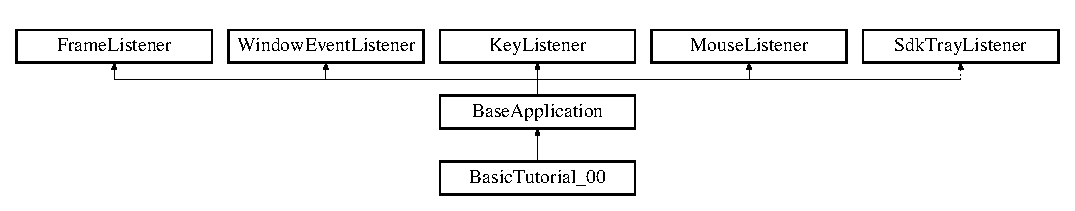
\includegraphics[height=2.382979cm]{class_base_application}
\end{center}
\end{figure}
\subsection*{Public Member Functions}
\begin{DoxyCompactItemize}
\item 
\mbox{\Hypertarget{class_base_application_a8a14a65a29118dd75173aa68678a05e1}\label{class_base_application_a8a14a65a29118dd75173aa68678a05e1}} 
virtual void {\bfseries go} (void)
\end{DoxyCompactItemize}
\subsection*{Protected Member Functions}
\begin{DoxyCompactItemize}
\item 
\mbox{\Hypertarget{class_base_application_a5853d0e148cb85b0297a6885e1d33a89}\label{class_base_application_a5853d0e148cb85b0297a6885e1d33a89}} 
virtual bool {\bfseries setup} ()
\item 
\mbox{\Hypertarget{class_base_application_a62ed46f90e9f82cc810997647a2c587e}\label{class_base_application_a62ed46f90e9f82cc810997647a2c587e}} 
virtual bool {\bfseries configure} (void)
\item 
\mbox{\Hypertarget{class_base_application_ad5bc9655041e1849a4c13f444a3712bd}\label{class_base_application_ad5bc9655041e1849a4c13f444a3712bd}} 
virtual void {\bfseries choose\+Scene\+Manager} (void)
\item 
\mbox{\Hypertarget{class_base_application_afa9d51527763cf9aee9cd4e1b1039d55}\label{class_base_application_afa9d51527763cf9aee9cd4e1b1039d55}} 
virtual void {\bfseries create\+Camera} (void)
\item 
\mbox{\Hypertarget{class_base_application_aff6fd9ff1ff0978cc68f19dd65be4778}\label{class_base_application_aff6fd9ff1ff0978cc68f19dd65be4778}} 
virtual void {\bfseries create\+Frame\+Listener} (void)
\item 
\mbox{\Hypertarget{class_base_application_aa97beeb4059b17d0ec22eae33286ec2d}\label{class_base_application_aa97beeb4059b17d0ec22eae33286ec2d}} 
virtual void {\bfseries create\+Scene} (void)=0
\item 
\mbox{\Hypertarget{class_base_application_a365146059b25391fe400f5fdb94f011e}\label{class_base_application_a365146059b25391fe400f5fdb94f011e}} 
virtual void {\bfseries destroy\+Scene} (void)
\item 
\mbox{\Hypertarget{class_base_application_a1f8f6730cae6ec769d8730b1af48486e}\label{class_base_application_a1f8f6730cae6ec769d8730b1af48486e}} 
virtual void {\bfseries create\+Viewports} (void)
\item 
\mbox{\Hypertarget{class_base_application_ae27301702f1e5de64619a39b1929f1f9}\label{class_base_application_ae27301702f1e5de64619a39b1929f1f9}} 
virtual void {\bfseries setup\+Resources} (void)
\item 
\mbox{\Hypertarget{class_base_application_a9b77972f0f747a61e1f8ceba2ad47641}\label{class_base_application_a9b77972f0f747a61e1f8ceba2ad47641}} 
virtual void {\bfseries create\+Resource\+Listener} (void)
\item 
\mbox{\Hypertarget{class_base_application_aaeb764e637dd87601a81a80156659d88}\label{class_base_application_aaeb764e637dd87601a81a80156659d88}} 
virtual void {\bfseries load\+Resources} (void)
\item 
\mbox{\Hypertarget{class_base_application_a03912a0f38b38fede7f08a2571e8fc56}\label{class_base_application_a03912a0f38b38fede7f08a2571e8fc56}} 
virtual bool {\bfseries frame\+Rendering\+Queued} (const Ogre\+::\+Frame\+Event \&evt)
\item 
\mbox{\Hypertarget{class_base_application_acfa977f04e435f18018ece805c1277ec}\label{class_base_application_acfa977f04e435f18018ece805c1277ec}} 
virtual bool {\bfseries key\+Pressed} (const O\+I\+S\+::\+Key\+Event \&arg)
\item 
\mbox{\Hypertarget{class_base_application_aba5c7c9dea7a0efc58b89310bae547e5}\label{class_base_application_aba5c7c9dea7a0efc58b89310bae547e5}} 
virtual bool {\bfseries key\+Released} (const O\+I\+S\+::\+Key\+Event \&arg)
\item 
\mbox{\Hypertarget{class_base_application_a126e59cb246b061e51eb6ce06a2ee8f4}\label{class_base_application_a126e59cb246b061e51eb6ce06a2ee8f4}} 
virtual bool {\bfseries mouse\+Moved} (const O\+I\+S\+::\+Mouse\+Event \&arg)
\item 
\mbox{\Hypertarget{class_base_application_a9255dfc1eabefd11c474ec45a6622504}\label{class_base_application_a9255dfc1eabefd11c474ec45a6622504}} 
virtual bool {\bfseries mouse\+Pressed} (const O\+I\+S\+::\+Mouse\+Event \&arg, O\+I\+S\+::\+Mouse\+Button\+ID id)
\item 
\mbox{\Hypertarget{class_base_application_aa102c5859c14c0690c749994a446b53d}\label{class_base_application_aa102c5859c14c0690c749994a446b53d}} 
virtual bool {\bfseries mouse\+Released} (const O\+I\+S\+::\+Mouse\+Event \&arg, O\+I\+S\+::\+Mouse\+Button\+ID id)
\item 
\mbox{\Hypertarget{class_base_application_afacf8a797588592ef0abbad593f10cfa}\label{class_base_application_afacf8a797588592ef0abbad593f10cfa}} 
virtual void {\bfseries window\+Resized} (Ogre\+::\+Render\+Window $\ast$rw)
\item 
\mbox{\Hypertarget{class_base_application_ae0e37ac54a31ff6e51d58c7654ad1b90}\label{class_base_application_ae0e37ac54a31ff6e51d58c7654ad1b90}} 
virtual void {\bfseries window\+Closed} (Ogre\+::\+Render\+Window $\ast$rw)
\end{DoxyCompactItemize}
\subsection*{Protected Attributes}
\begin{DoxyCompactItemize}
\item 
\mbox{\Hypertarget{class_base_application_add84ba707dc6c57e6283f214b1274110}\label{class_base_application_add84ba707dc6c57e6283f214b1274110}} 
Ogre\+::\+Root $\ast$ {\bfseries m\+Root}
\item 
\mbox{\Hypertarget{class_base_application_a3829c6b12afe911e97e6b4524b33a38b}\label{class_base_application_a3829c6b12afe911e97e6b4524b33a38b}} 
Ogre\+::\+Camera $\ast$ {\bfseries m\+Camera}
\item 
\mbox{\Hypertarget{class_base_application_a8a7684f4f9a57ed3089048ad1a913b2d}\label{class_base_application_a8a7684f4f9a57ed3089048ad1a913b2d}} 
Ogre\+::\+Scene\+Manager $\ast$ {\bfseries m\+Scene\+Mgr}
\item 
\mbox{\Hypertarget{class_base_application_ac5d8e9c81e036897bc82f81eff8c570f}\label{class_base_application_ac5d8e9c81e036897bc82f81eff8c570f}} 
Ogre\+::\+Render\+Window $\ast$ {\bfseries m\+Window}
\item 
\mbox{\Hypertarget{class_base_application_a765e0df01c141a16df3178ab4f17afe6}\label{class_base_application_a765e0df01c141a16df3178ab4f17afe6}} 
Ogre\+::\+String {\bfseries m\+Resources\+Cfg}
\item 
\mbox{\Hypertarget{class_base_application_a04f2fe47fa164fd78d986dc0df70b7fb}\label{class_base_application_a04f2fe47fa164fd78d986dc0df70b7fb}} 
Ogre\+::\+String {\bfseries m\+Plugins\+Cfg}
\item 
\mbox{\Hypertarget{class_base_application_a7faa397f4f4861ee8c361a01e90b4416}\label{class_base_application_a7faa397f4f4861ee8c361a01e90b4416}} 
Ogre\+Bites\+::\+Sdk\+Tray\+Manager $\ast$ {\bfseries m\+Tray\+Mgr}
\item 
\mbox{\Hypertarget{class_base_application_a9ae38dea6316058549151fff66a91fcd}\label{class_base_application_a9ae38dea6316058549151fff66a91fcd}} 
Ogre\+Bites\+::\+Sdk\+Camera\+Man $\ast$ {\bfseries m\+Camera\+Man}
\item 
\mbox{\Hypertarget{class_base_application_a6a11054ca61efdf558e0ff1b2de43a12}\label{class_base_application_a6a11054ca61efdf558e0ff1b2de43a12}} 
Ogre\+Bites\+::\+Params\+Panel $\ast$ {\bfseries m\+Details\+Panel}
\item 
\mbox{\Hypertarget{class_base_application_ac7e861799862cb645f1d78b170aef80d}\label{class_base_application_ac7e861799862cb645f1d78b170aef80d}} 
bool {\bfseries m\+Cursor\+Was\+Visible}
\item 
\mbox{\Hypertarget{class_base_application_a755f26d3a9915aaf830750d877e39d86}\label{class_base_application_a755f26d3a9915aaf830750d877e39d86}} 
bool {\bfseries m\+Shut\+Down}
\item 
\mbox{\Hypertarget{class_base_application_abc9503c8462e225b5d0d55c952d9e4a9}\label{class_base_application_abc9503c8462e225b5d0d55c952d9e4a9}} 
O\+I\+S\+::\+Input\+Manager $\ast$ {\bfseries m\+Input\+Manager}
\item 
\mbox{\Hypertarget{class_base_application_add9b97fbe64da2814d3af113bac58c43}\label{class_base_application_add9b97fbe64da2814d3af113bac58c43}} 
O\+I\+S\+::\+Mouse $\ast$ {\bfseries m\+Mouse}
\item 
\mbox{\Hypertarget{class_base_application_a9d6e19cf50c47379fbaae55bff28079c}\label{class_base_application_a9d6e19cf50c47379fbaae55bff28079c}} 
O\+I\+S\+::\+Keyboard $\ast$ {\bfseries m\+Keyboard}
\end{DoxyCompactItemize}


The documentation for this class was generated from the following files\+:\begin{DoxyCompactItemize}
\item 
source/Base\+Application.\+h\item 
source/Base\+Application.\+cpp\end{DoxyCompactItemize}

\hypertarget{class_basic_tutorial__00}{}\section{Basic\+Tutorial\+\_\+00 Class Reference}
\label{class_basic_tutorial__00}\index{Basic\+Tutorial\+\_\+00@{Basic\+Tutorial\+\_\+00}}


3D Game Programming ~\newline
My Name\+: �B �� �� ~\newline
My ID\+: 0656124 ~\newline
My Email\+: \href{mailto:ciaskbe@gmail.com}{\tt ciaskbe@gmail.\+com} ~\newline
 Date\+: 2017/10/11  




{\ttfamily \#include $<$Tutorial\+Application.\+h$>$}

Inheritance diagram for Basic\+Tutorial\+\_\+00\+:\begin{figure}[H]
\begin{center}
\leavevmode
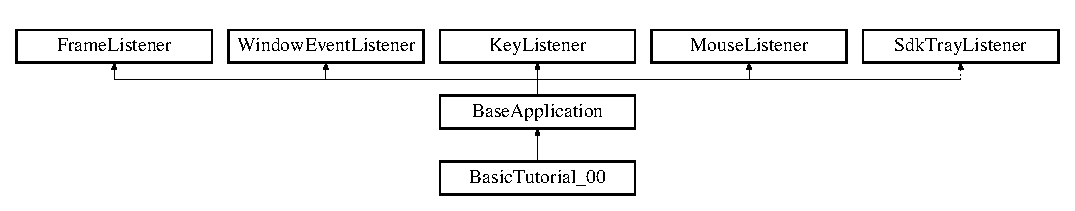
\includegraphics[height=2.382979cm]{class_basic_tutorial__00}
\end{center}
\end{figure}
\subsection*{Public Member Functions}
\begin{DoxyCompactItemize}
\item 
\mbox{\Hypertarget{class_basic_tutorial__00_adc2454d9f8226e0958ecf702f355846e}\label{class_basic_tutorial__00_adc2454d9f8226e0958ecf702f355846e}} 
virtual void {\bfseries create\+Viewports} (void)
\item 
\mbox{\Hypertarget{class_basic_tutorial__00_a15a3d4673724ec99077ce992f996a550}\label{class_basic_tutorial__00_a15a3d4673724ec99077ce992f996a550}} 
virtual void {\bfseries create\+Scene} (void)
\item 
\mbox{\Hypertarget{class_basic_tutorial__00_a1bf709417d654dffc2ea10987412b912}\label{class_basic_tutorial__00_a1bf709417d654dffc2ea10987412b912}} 
virtual void {\bfseries create\+Camera} (void)
\item 
\mbox{\Hypertarget{class_basic_tutorial__00_aba97a29d983586d2dc8e108d3bccf721}\label{class_basic_tutorial__00_aba97a29d983586d2dc8e108d3bccf721}} 
virtual void {\bfseries choose\+Scene\+Manager} (void)
\item 
\mbox{\Hypertarget{class_basic_tutorial__00_a94e281a96584a25bf57b1c5e73737c81}\label{class_basic_tutorial__00_a94e281a96584a25bf57b1c5e73737c81}} 
virtual bool {\bfseries frame\+Started} (const Ogre\+::\+Frame\+Event \&evt)
\end{DoxyCompactItemize}
\subsection*{Protected Member Functions}
\begin{DoxyCompactItemize}
\item 
void \hyperlink{class_basic_tutorial__00_a6d4684502f2f7b2cf628a975d7750d8e}{create\+Viewport\+\_\+00} (void)
\begin{DoxyCompactList}\small\item\em Create a viewport. \end{DoxyCompactList}\item 
\mbox{\Hypertarget{class_basic_tutorial__00_a2801a2f0d91d80b471da48344d2ccccf}\label{class_basic_tutorial__00_a2801a2f0d91d80b471da48344d2ccccf}} 
void {\bfseries create\+Viewport\+\_\+01} (void)
\item 
\mbox{\Hypertarget{class_basic_tutorial__00_a3479c50dbf8dc06a7ea77014eb94c6e7}\label{class_basic_tutorial__00_a3479c50dbf8dc06a7ea77014eb94c6e7}} 
void {\bfseries create\+Camera\+\_\+00} ()
\item 
\mbox{\Hypertarget{class_basic_tutorial__00_a8745a127adeb69fa769f832fd41412c0}\label{class_basic_tutorial__00_a8745a127adeb69fa769f832fd41412c0}} 
void {\bfseries create\+Camera\+\_\+01} ()
\item 
\mbox{\Hypertarget{class_basic_tutorial__00_aa84173e509858146cbfb98274c1ef56e}\label{class_basic_tutorial__00_aa84173e509858146cbfb98274c1ef56e}} 
void {\bfseries create\+Scene\+\_\+00} ()
\item 
\mbox{\Hypertarget{class_basic_tutorial__00_aad14e1ca565797c4b7dcff31bc0e1494}\label{class_basic_tutorial__00_aad14e1ca565797c4b7dcff31bc0e1494}} 
void {\bfseries create\+Scene\+\_\+01} ()
\item 
\mbox{\Hypertarget{class_basic_tutorial__00_adc1a0b32d78b1980b3ee51a1b1e1e69b}\label{class_basic_tutorial__00_adc1a0b32d78b1980b3ee51a1b1e1e69b}} 
bool {\bfseries key\+Pressed} (const O\+I\+S\+::\+Key\+Event \&arg)
\item 
\mbox{\Hypertarget{class_basic_tutorial__00_aacca7a0a2a5a0e0d007b9c6c30b4941b}\label{class_basic_tutorial__00_aacca7a0a2a5a0e0d007b9c6c30b4941b}} 
bool {\bfseries key\+Released} (const O\+I\+S\+::\+Key\+Event \&arg)
\end{DoxyCompactItemize}
\subsection*{Protected Attributes}
\begin{DoxyCompactItemize}
\item 
\mbox{\Hypertarget{class_basic_tutorial__00_a6676a92b50e9b43634d4c66488537b73}\label{class_basic_tutorial__00_a6676a92b50e9b43634d4c66488537b73}} 
Ogre\+::\+Viewport $\ast$ {\bfseries m\+Viewport\+Arr} \mbox{[}8\mbox{]}
\item 
\mbox{\Hypertarget{class_basic_tutorial__00_af8d457d912286a98c0975c52d4faf910}\label{class_basic_tutorial__00_af8d457d912286a98c0975c52d4faf910}} 
Ogre\+::\+Camera $\ast$ {\bfseries m\+Camera\+Arr} \mbox{[}8\mbox{]}
\item 
\mbox{\Hypertarget{class_basic_tutorial__00_a603779b6087698c57b7989e16d8a9b93}\label{class_basic_tutorial__00_a603779b6087698c57b7989e16d8a9b93}} 
Ogre\+::\+Scene\+Manager $\ast$ {\bfseries m\+Scene\+Mgr\+Arr} \mbox{[}8\mbox{]}
\item 
\mbox{\Hypertarget{class_basic_tutorial__00_a700c07f924c71e9fa1885a46f599d934}\label{class_basic_tutorial__00_a700c07f924c71e9fa1885a46f599d934}} 
Ogre\+Bites\+::\+Sdk\+Camera\+Man $\ast$ {\bfseries m\+Camera\+Man\+Arr} \mbox{[}8\mbox{]}
\item 
\mbox{\Hypertarget{class_basic_tutorial__00_ac8d1030aab352cecd5ccd6234b5573f5}\label{class_basic_tutorial__00_ac8d1030aab352cecd5ccd6234b5573f5}} 
bool {\bfseries animation\+\_\+state}
\item 
\mbox{\Hypertarget{class_basic_tutorial__00_a060eadaf0a23ee7a6a928d9b1df0d5f9}\label{class_basic_tutorial__00_a060eadaf0a23ee7a6a928d9b1df0d5f9}} 
Ogre\+::\+Vector3 {\bfseries acceleration}
\item 
\mbox{\Hypertarget{class_basic_tutorial__00_a9146709112187aa671a6a6dbe3282556}\label{class_basic_tutorial__00_a9146709112187aa671a6a6dbe3282556}} 
Ogre\+::\+Vector3 {\bfseries velocity}
\end{DoxyCompactItemize}


\subsection{Detailed Description}
3D Game Programming ~\newline
My Name\+: �B �� �� ~\newline
My ID\+: 0656124 ~\newline
My Email\+: \href{mailto:ciaskbe@gmail.com}{\tt ciaskbe@gmail.\+com} ~\newline
 Date\+: 2017/10/11 

This is an assignment of 3D Game Programming 

\subsection{Member Function Documentation}
\mbox{\Hypertarget{class_basic_tutorial__00_a6d4684502f2f7b2cf628a975d7750d8e}\label{class_basic_tutorial__00_a6d4684502f2f7b2cf628a975d7750d8e}} 
\index{Basic\+Tutorial\+\_\+00@{Basic\+Tutorial\+\_\+00}!create\+Viewport\+\_\+00@{create\+Viewport\+\_\+00}}
\index{create\+Viewport\+\_\+00@{create\+Viewport\+\_\+00}!Basic\+Tutorial\+\_\+00@{Basic\+Tutorial\+\_\+00}}
\subsubsection{\texorpdfstring{create\+Viewport\+\_\+00()}{createViewport\_00()}}
{\footnotesize\ttfamily void Basic\+Tutorial\+\_\+00\+::create\+Viewport\+\_\+00 (\begin{DoxyParamCaption}\item[{void}]{ }\end{DoxyParamCaption})\hspace{0.3cm}{\ttfamily [protected]}}



Create a viewport. 

Create a viewport for the entire screen.

\begin{DoxyReturn}{Returns}
The sum of two integers. 
\end{DoxyReturn}


The documentation for this class was generated from the following files\+:\begin{DoxyCompactItemize}
\item 
source/Tutorial\+Application.\+h\item 
source/Tutorial\+Application.\+cpp\end{DoxyCompactItemize}

%--- End generated contents ---

% Index
\backmatter
\newpage
\phantomsection
\clearemptydoublepage
\addcontentsline{toc}{chapter}{Index}
\printindex

\end{document}
